% Author: Izaak Neutelings (June, 2018)
\documentclass[border=3pt,tikz]{standalone}
\usepackage{tikz}
\usetikzlibrary{arrows.meta} % to control arrow size
\tikzset{>={Latex[length=4,width=4]}} % for LaTeX arrow head
\usetikzlibrary{calc}
\usepackage{amsmath,bm}
\usepackage{relsize} % for fontsize
\usepackage{xcolor} % for colored text

\colorlet{mylightblue}{blue!5!white}
\colorlet{mydarkblue}{blue!30!black}
\colorlet{myblue}{blue!50!black}
\colorlet{myred}{red!50!black}
\colorlet{mydarkred}{red!30!black}
\colorlet{mydarkgreen}{green!30!black}

\def\str{\vrule height 9pt depth 2pt width 0pt} % strut

\begin{document}


% FLOW CHART
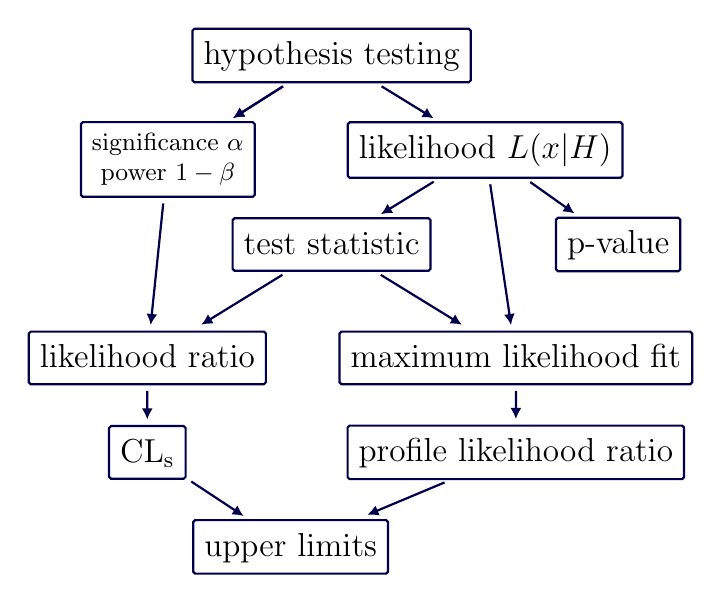
\begin{tikzpicture}[xscale=1.3,yscale=1.2,
                    fscale/.style={font=\relsize{#1}},
                    arrow/.style={->,thick,mydarkblue,shorten <=2,shorten >=2},
                    sarrow/.style={->,thick,mydarkblue,shorten <=2,shorten >=4}]
  
  \def\topic(#1,#2,#3,#4){
    \node[draw=mydarkblue,fill=white,thick,rounded corners=0.7,inner sep=4]
      (#1) at (#2,#3) [fscale=1.2,align=center] {#4};
  }
  
  % TOPICS
  \topic(HT,     0,    0,  \str hypothesis testing)
  \topic(LH,   1.5, -1.0,  \str {likelihood ${L(x|H)}$})
  \topic(TS,   0.0, -2.0,  \str test statistic)
  %\topic(CR,  -1.5, -1.0,  \str critical region)
  \topic(SP,  -1.6, -1.1,  \small significance $\alpha$\\[-3pt]\small power $1-\beta$)
  \topic(PV,   2.8, -2.0,  \str p-value)
  \topic(LR,  -1.8, -3.2,  \str likelihood ratio)
  \topic(CLs, -1.8, -4.2,  \str CL$_\text{s}$)
  \topic(PLR,  1.8, -4.2,  \str profile likelihood ratio)
  \topic(MLF,  1.8, -3.2,  \str maximum likelihood fit)
  \topic(UL,  -0.4, -5.2,  \str upper limits)
  
  % ARROW
  \draw[arrow,->] (HT)  -- (LH);
  \draw[arrow,->] (HT)  -- (SP);
  \draw[arrow,->] (SP)  -- (LR);
  \draw[arrow,->] (LH)  -- (MLF);
  \draw[arrow,->] (LH)  -- (TS);
  \draw[arrow,->] (LH)  -- (PV);
  \draw[arrow,->] (HT)  -- (SP);
  \draw[sarrow,->] (TS)  -- (LR);
  \draw[sarrow,->] (TS)  -- (MLF);
  \draw[arrow,->] (MLF) -- (PLR);
  \draw[arrow,->] (LR)  -- (CLs);
  \draw[arrow,->] (CLs) -- (UL);
  \draw[sarrow,->] (PLR) -- (UL);
  
\end{tikzpicture}



\end{document}
